% ----------------------------------------------------------
% DESENVOLVIMENTO   
% ----------------------------------------------------------
\chapter{Desenvolvimento} \label{cha:desenvolvimento}

É a parte principal do texto. Apresenta o assunto, fundamentação teórica, metodologia (materiais e métodos), os resultados e as respectivas discussões traçando relações com os trabalhos analisados na revisão de literatura.


\section{Revisão da Literatura}

É uma análise comentada sobre o que já foi publicado sobre o assunto da pesquisa, buscando mostrar os pontos de vista convergentes e divergentes entre os autores. Traça-se um quadro teórico e elabora-se a estruturação conceitual que subsidiará o desenvolvimento da pesquisa. A revisão de literatura permitirá um mapeamento de quem já escreveu e o que já foi escrito sobre o assunto ou o problema de pesquisa.

\subsection{Título da seção terciária}

As políticas públicas são princípios norteadores, diretrizes para ações do 
poder público para com a sociedade. Faz-se necessário para tanto o seu 
entendimento, para Teixeira (2002, p. 2, aspas do autor),

\begin{citacao}
As citações diretas, no texto, com mais de três linhas, devem ser
destacadas com recuo de 4 cm da margem esquerda, com letra menor que a do texto
utilizado e sem as aspas. No caso de documentos datilografados, deve-se
observar apenas o recuo \cite[5.3]{NBR10520:2002}.
\end{citacao}

Neste entendimento percebe-se a importância da existência das políticas 

\subsubsection{Título da seção quaternária}

As ilustrações (fotografias, gráficos, mapas, plantas, quadros) e tabelas 
devem ser citados e inseridos o mais próximo possível do trecho a que se referem. 

Texto texto texto texto texto texto texto texto texto texto texto texto texto texto texto 
texto, conforme o Figura \ref{fig:figura1} e \ref{fig:gráfico1}.

\begin{figure}[htb]
	\caption{\label{fig:figura1}Organização de um trabalho acadêmico com os elementos pré-textuais, textuais e pós textuais}
	\begin{center}
	    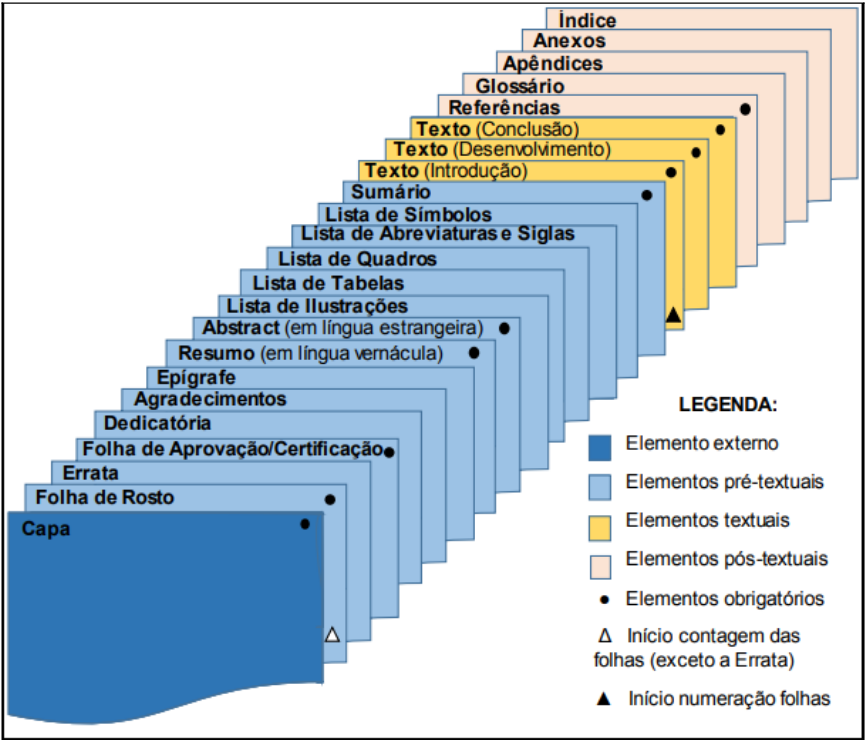
\includegraphics[scale=0.5]{imagens/figura1.png}
	\end{center}
	\legend{Fonte: elaborada pelos autores, 2026}
\end{figure}



Texto texto texto texto texto texto texto texto texto texto texto texto texto texto 
texto texto texto texto texto texto texto texto texto texto texto texto texto texto texto 
texto texto texto texto texto texto texto texto texto texto texto texto texto texto texto 
texto texto. 

\begin{figure}[htb]
	\caption{ \label{fig:gráfico1}Gráfico de Distribuição do número de matrículas por etapas da educação básica município de Avaré – 2014}
	\begin{center}
	    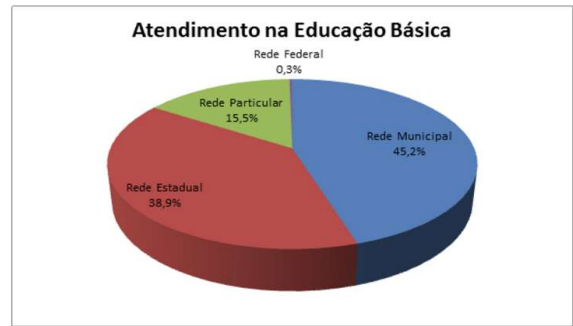
\includegraphics[scale=1.0]{imagens/grafs_1.png}
	\end{center}
	\legend{Fonte: Secretaria Municipal de Educação de Avaré (2014). }
\end{figure}

	

\setcounter{secnumdepth}{4}